% \documentclass[rnd]{mas_proposal}
\documentclass[thesis]{mas_proposal}

\usepackage[utf8]{inputenc}
\usepackage{amsmath}
\usepackage{amsfonts}
\usepackage{hyperref}
\usepackage{amssymb}
\usepackage{graphicx}

\title{Out of distribution detection in 3D semantic segmentation}
\author{Lokesh Veeramacheneni}
\supervisors{Prof. Dr. Paul G Pl\"{o}ger\\ Dr. Matias Valdenegro Toro \\ Prof. Dr. Sebastian Houben }
\date{October 2021}

\thirdpartylogo{images/DFKI}

\begin{document}

\maketitle

\pagestyle{plain}

\section{Introduction}
% \begin{itemize}
%     \item An introduction to the general topic you are covering.
%     \item Why is it important?
% \end{itemize}
Many robotic \cite{thrun2006stanley} \cite{patz2008practical}, autonomous driving \cite{li2016vehicle} systems deployed in the real world, dynamic environments now use LiDAR as the primary sensor.
The 3D LiDAR data acquired offers a true-size replica of rich 3D geometry and can be represented as a 3D point cloud format or using 2D grids. eg: range image representation \cite{Milioto2019}.
Semantic scene understanding is one of the key components of autonomous driving systems. 
Semantic segmentation is an important task in semantic scene understanding.
Semantic segmentation requires the labelling of each data point (3D point in LiDAR/pixel in camera) with its corresponding class.

The existing models for 3D semantic segmentation are insanely complex and uncertain about their detections \cite{bhandary2020evaluating}. 
This uncertainty in addition to input as out of distribution (OOD) objects questions the safety and performance of the models.
One such real-world example is Tesla autopilot stops after misdetecting a billboard with "STOP" written on it as a traffic stop sign \cite{tesla_fails}. 
Another such failure is the same autopilot detecting the moon as a yellow sign and slows the car \cite{tesla_fails}.
In all the above scenarios, the model is unable to detect the object as OOD and resulting in undesired outcomes.
\cite{liang2017enhancing_ODIN}, \cite{bevandic2018discriminative}, \cite{Robinchan_2021_ICCV}, and \cite{angus2019_pixellevelOOD} define OOD as the input classes which
are not included in the training set. This is because most of the training sets of
datasets were assumed as a closed world that is the predictions are made on the
predefined set of classes. When deployed in the real world the autonomous agent will
encounter a new class which leads to dangerous situations as specified in the above
example which is still an unsolved problem.
\begin{figure}[h]
    \centering
    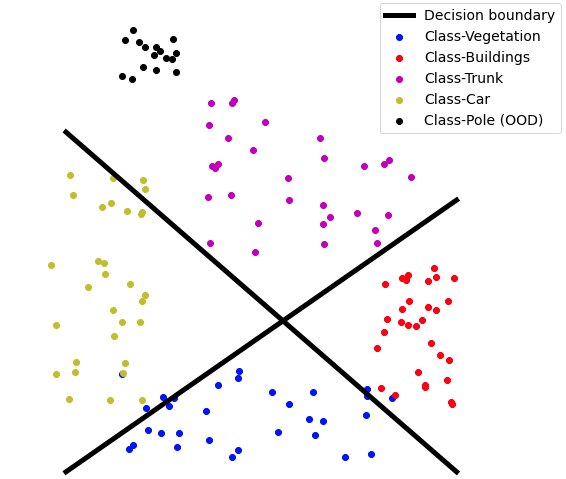
\includegraphics[scale=0.5]{images/OOD.png}
    \caption{Representation of the semantic space with the decision boundaries of four classes in training set in colour and the points in black are of OOD}
    \label{fig:semantic_space}
\end{figure}
Figure \ref{fig:semantic_space} displays an example semantic
space with decision boundaries between four classes in the training set and one OOD
class represented in black. The training classes were vegetation, buildings, trunk
and car, whereas the OOD class is a pole. During inference, the pole class is classified
as trunk which is a wrong prediction. The ideal behaviour of the classifier is to specify
this is an unknown class object and thus probably request for human input. In
this thesis, we will try to extend the classifier to detect these unknown objects by
exploring OOD detection methods and also quantified uncertainty.

A decade long study has been performed on the task of semantic segmentation, \cite{ZHU201612} refers to all the traditional approaches based on handcrafted features.
With the advent of deep learning, a richer feature representation led to mapping input to semantic labels as an end to end procedure.
The most popular 3D semantic segmentation datasets in the context of autonomous driving are Semantic KITTI \cite{Behley_2019_ICCV}, nuScenes-lidarSeg \cite{caesar2020nuscenes} and Sydney Urban \cite{de2013unsupervised} collected by various sensors are publicly available.
3D semantic segmentation datasets are limited in size and diversity because labelling is intensive and requires special skills to handle.

There are a diverse range of methods for the task of 3D semantic segmentation. 
They inlcude point based methods such as PointNet++ \cite{qi2017pointnet++}, RandLA-Net \cite{Hu_2020_CVPR_Randla}, and many more.
There also exists image based methods which employ various projection algorithms and popular methods in this segment include SqueeseSegV3 \cite{Sequesesegv3_2018}, RangeNet++ \cite{Milioto2019}, and SalsaNext \cite{SalsaNext_2020}.
Graph-based and Voxel-based methods are some of their kind to solve the task of 3D semantic segmentation.
In the later sections, we will discuss the problem statement, corresponding related work and project plan.


\subsection{Problem Statement}
% \begin{itemize}
%     \item What are you going to solve?
%     \item How are you evaluating?
% \end{itemize}
In this thesis, we study the application of out of distribution (OOD) detection over the 3D semantic segmentation problem in the context of autonomous driving.
Notably, we study the 3D semantic segmentation datasets available and create a benchmark for in and out distribution for the OOD setting.

The other major issue, we address in this thesis is the OOD detection methods themselves.
Existing OOD detection methods are developed on 2D classification tasks and the study of these methods on 3D semantic segmentation tasks is not yet studied. 
This study is also challenging because the existing OOD methods are not easily adaptable to the 3D segmentation models becasue segmentation involves multi class classification and moreover high dimensionality of the 3D data.
\newline

The research questions answered by this thesis are:
\begin{itemize}
    \item[\textbf{R1}] How to create a benchmark over 3D segmentation datasets for the OOD setting? i.e., create the in and out distribution datasets.
    \item[\textbf{R2}] How to extend current OOD detection methods from 2D classification task to 3D semantic segmentation?
    \item[\textbf{R3}] Is uncertainty quantification an effective approach to classify the OOD detection in 3D semantic segmentation models?
    % \item[\textbf{R4}] What metrics can be applied for the OOD detection task over 3D semantic segmentation models? 
    \item[\textbf{R4}] How to evaluate the OOD detections over the 3D semantic segmentation task?
\end{itemize}
\section{Related Work}
% \begin{itemize}
%     \item What have other people done?
%     \item Why is it not sufficient?
% \end{itemize}
In this related work, we discuss the methods involving 3D semantic segmentation, out of distribution (OOD) detection methods and performance metrics available.

\subsection{3D semantic segmentation}
The existing deep learning methods for 3D semantic segmentation is be divided into 4 types based on their mode of input.
The first one is point-based methods, these type of methods perform operations directly on the raw point clouds. 
These type of methods are more popular and vastly used.
Some of the well-known methods in this category are PointNet \cite{Qi_2017_CVPR_pointnet}, PointNet++ \cite{qi2017pointnet++}, RandLA-Net \cite{Hu_2020_CVPR_Randla}, SPLATNet \cite{Su_2018_CVPR_splatnet}, TangentConvolution \cite{Tatarchenko_2018_CVPR_tangconv}, ShellNet \cite{Zhang_2019_ICCV_shellnet}, PointCNN \cite{li2018pointcnn}.

The second most kind of deep learning method for 3D semantic segmentation is Image-based methods.
These methods require the projection of the 3D point clouds into range images or multi-view images. 
This projection allows these methods to employ well developed and advanced 2D semantic segmentation methods like (cite).
Popular methods in this category include SqueeseSegV3 \cite{Sequesesegv3_2018}, RangeNet++ \cite{Milioto2019}, 3D-MiniNet \cite{3Dmininet}, SalsaNext \cite{SalsaNext_2020}, LiSeg \cite{liseg}, KPRNet \cite{kochanov2020kprnet} use range image representation.

The other two kinds of methods are voxel-based methods and graph-based methods. 
Voxel-based methods require a small preprocessing of converting raw point clouds to voxels.
Some methods using voxels are 3D U-Net \cite{3Dmininet}, Cylinder3D \cite{zhou2020cylinder3d}. 
Dynamic graph CNN \cite{dyn_graph_cnn}, GAC Net \cite{Wang_2019_CVPR_GACNet} are few graph-based methods available.

There exists a few open 3D LiDAR semantic segmentation datasets. 
Oakland \cite{oakland}, TUM city campus \cite{gehrung2017approach_tum_campus}, Semantic3D \cite{hackel2017semantic3d}, Paris-lille-3D \cite{roynard2018paris}, S3DIS \cite{Armeni_2016_CVPR_S3DIS} are a few datasets with static LiDAR and has point annotations.
The other type of datasets includes sequential data.
These type of datasets include Semantic KITTI \cite{Behley_2019_ICCV}, A2D2 \cite{geyer2020a2d2}, nuScenes-lidarSeg \cite{caesar2020nuscenes}, KITTI-360 \cite{Xie_2016_CVPR_KITTI_360}, Sydney Urban \cite{de2013unsupervised} and they have point annotations.
There also exist 3D box annotations with sequential data and they are KITTI \cite{KITTI}, H3D \cite{H3D}, and DENSE \cite{Bijelic_2020_CVPR_DENSE}. %Waymo \cite{Sun_2020_CVPR_Waymo}, 
GTA-V \cite{GTAV} and SynthCity \cite{griffiths2019synthcity} are only a few synthetic datasets available for 3D semantic segmentation.

\subsection{OOD detection}
The OOD detection methods are broadly divided into the threshold, non-threshold, uncertainty and generative based methods.
Generative methods will not be studied in this thesis because these methods are out of the scope of the project.
All the OOD methods discussed below are evaluated on the 2D classification task and no approach was deduced for the 3D semantic segmentation task.
\subsubsection{Threshold based}
These methods employ a threshold-based detector.
The well-known OOD detector is Maximum Softmax Probability (MSP) proposed in \cite{hendrycks2016baseline_MSP}. 
This method considers the max of the softmax output and decides an OOD based on the confidence threshold.
Since the softmax scores can be overconfident \cite{liang2017enhancing_ODIN} proposed ODIN which uses calibrated confidence score which uses temperature scaling.
Apart from calibrated confidence score, ODIN also makes use of noise perturbations in input.
Combining these two, a threshold-based detector is applied at the end. 
\cite{lee2018simple_mahalanobis} proposed Mahalanobis distance as a confidence score. 
In addition to this score, input perturbations were also added. 
The score is calculated at all layers then ensembled and given to threshold based detector.
\subsubsection{Non-threshold based}
\cite{hendrycks2018deep_OE} proposed Outlier Exposure which makes use of a large, unlabeled auxiliary dataset to improve the OOD detection performance. 
Then a new classifier is utilized with a distinct objective function. 
\cite{chen2020robust} proposes a novel method for improvement of robustness of OOD detection called Adversarial Learning with inlier and Outlier Exposure (ALOE) which served as an extension to Outlier Exposure proposed by \cite{hendrycks2018deep_OE}.
\subsubsection{Uncertainty based}
\cite{lakshminarayanan2016simple} uses ensembled models to evaluate epistemic uncertainty and utilizes predictive entropy to clasify the in distribution and out of distribution samples.
\cite{pmlr-v119-van-amersfoort20a} uses a novel radial basis function approach to calculate the epistemic uncertainty and argues OOD can be detected using epistemic uncertainty.
The above methods evaluate the uncertainty on 2D models, there exists only \cite{bhandary2020evaluating} which apply the deep ensemble technique, Dropout and Dropconnet to the 3D semantic segmentation models to evaluate the uncertainty.

\subsection{Metrics for OOD detection}
There are a few metrics that deal with OOD detection and they include
\subsubsection{Area Under Receiver Operating characteristic Curve (AUROC)}
AUROC portrays the discrimination ability of the model between positive and negative cases. 
It is calculated as the area under the ROC curve which in turn is calculated from true positive rate (TPR) and false-positive rate (FPR) across various decision thresholds.
The value of AUROC ranges between 0.0 and 1.0 with 0.5 being worst (random classifier) and 1.0 being best.
\subsubsection{Area Under Precision-Recall Curve (AUPRC)}
The area under the PR curve is calculated as AUPRC. 
PR curve shows the tradeoff between various thresholded precision and recall.
The interpretation of AUPRC is trickier than AUROC. 
In AUROC the baseline is 0.5 as its random classifier but for AUPRC its fraction of positives ($\frac{positve\ examples}{total\ examples}$).
This implies that various classes have various baseline AUPRC values.
\subsubsection{FPR at 95\% TPR}
This metric calculates the FPR on OOD samples when the TPR is at 95\% in distribution samples.
\subsubsection{mean intersection-over-union (mIOU)}
The metrics discussed till now evaluate the performance on OOD detection, but this metric is used to evaluate the performance of the 3D semantic segmentation model.
It is calculated as IOU over all the classes and it is given by
$$
    mIOU=\frac{1}{C} \sum_{x=1}^C \frac{TP_x}{TP_x + FP_x + FN_x}
$$
where C is the number of classes and $TP_x, FP_x, FN_x$ are the true positives, false positives and false negatives of class x.

\section{Project Plan}
In this section, the project plan including work packages, tasks and timeline for each task is proposed.
\subsection{Work Packages}
The bare minimum will include the following packages:
\begin{enumerate}
    \item[WP1] Literature Search
    \begin{itemize}
        \item[-] Literature search on the existing 3D datasets on semantic segmentation for benchmarking.
        \item[-] Literature search on the existing  3D models for semantic segementation.
        \item[-] Literature search over the out of distribution methods.
        % \item[-] Documentation.
    \end{itemize} 
    \item[WP2] Dataset OOD benchmark proposal
    \begin{itemize}
        \item[-] 3D semantic segmentation dataset collection for benchmarking.
        \item[-] Benchmark datasets for in-distribution and out-distribution.
        % \item[-] Documentation.
    \end{itemize}
    \item[WP3] Experimentation
    \begin{itemize}
        \item[-] Extend an existing 3D semantic segmentation model as baseline model for out of distribution detection problem.
        \item[-] Extend the state of the art (SOTA) 3D semantic segmentation model for out of distribution detection problem.
        % \item[-] Extend the implemented 3D model (baseline and SOTA) to out of distribution detection problem.
        % \item[-] Documentation. 
    \end{itemize}
    \item[WP4] Evaluation
    \begin{itemize}
        \item[-] Evaluate the baseline model and SOTA model on the proposed evaluation methods.
        \item[-] Compare both the model on OOD detection
        % \item[-] Documentation
    \end{itemize} 
    \item[WP5] Project Report
    \begin{itemize}
        % \item[-] Update and review existing report sections (literature, datasets, experimentation and evaluation)
        % \item[-] Report completion and submission
        \item[-] Write the report
    \end{itemize} 
\end{enumerate}
% Keep in mind that depending on your project, you will probably need to add work packages that are more suited to your projects.

\subsection{Milestones}
\begin{enumerate}
    \item[M1] Literature search
    \item[M2] Dataset benchmarking
    \item[M3] Models implementation
    \item[M4] Evaluation and comparison
    \item[M5] Report submission
\end{enumerate}



\subsection{Deliverables}
\subsubsection*{Minimum Viable}

\begin{itemize}
    \item Systematic literature survey of methods over
        \subitem- Datasets in 3D semantic segmentation
        \subitem- Existing out of distribution methods 
        \subitem- Semantic segmentation models on 3D datasets
    \item Proposal of benchmarking datasets for out of distribution detection in 3D semantic
    segmentation
    \item Study of uncertainty quantification in 3D semantic segmentation models
    \item Implementation of method which uses quantified uncertainty for OOD detection
\end{itemize}

\subsubsection*{Expected}
\begin{itemize}
    \item Systematic evaluation of the implemented OOD detection method over the
    proposed dataset
    \item Extension of the state of the art model for OOD detection
    \item Evaluation and comparison of the extended state of the art model to baseline algorithm
\end{itemize}

\subsubsection*{Desired}
\begin{itemize}
    % \item Evaluation and comparison of the extended state of the art model to baseline algorithm
    % \item Draft a research paper with the insights/findings from thesis
    \item Proposal of a refinement over the current OOD model for higher performance
\end{itemize}

\subsection{Project Schedule}
% Include a gantt chart here. It doesn't have to be detailed, but it should include the milestones you mentioned above.
% Make sure to include the writing of your report throughout the whole project, not just at the end.
The detailed plan of tasks in duration of 6 months of thesis is given in figure 1.

\begin{figure}[h!]
    \caption{Illustration of project timeline over the period of six months}
    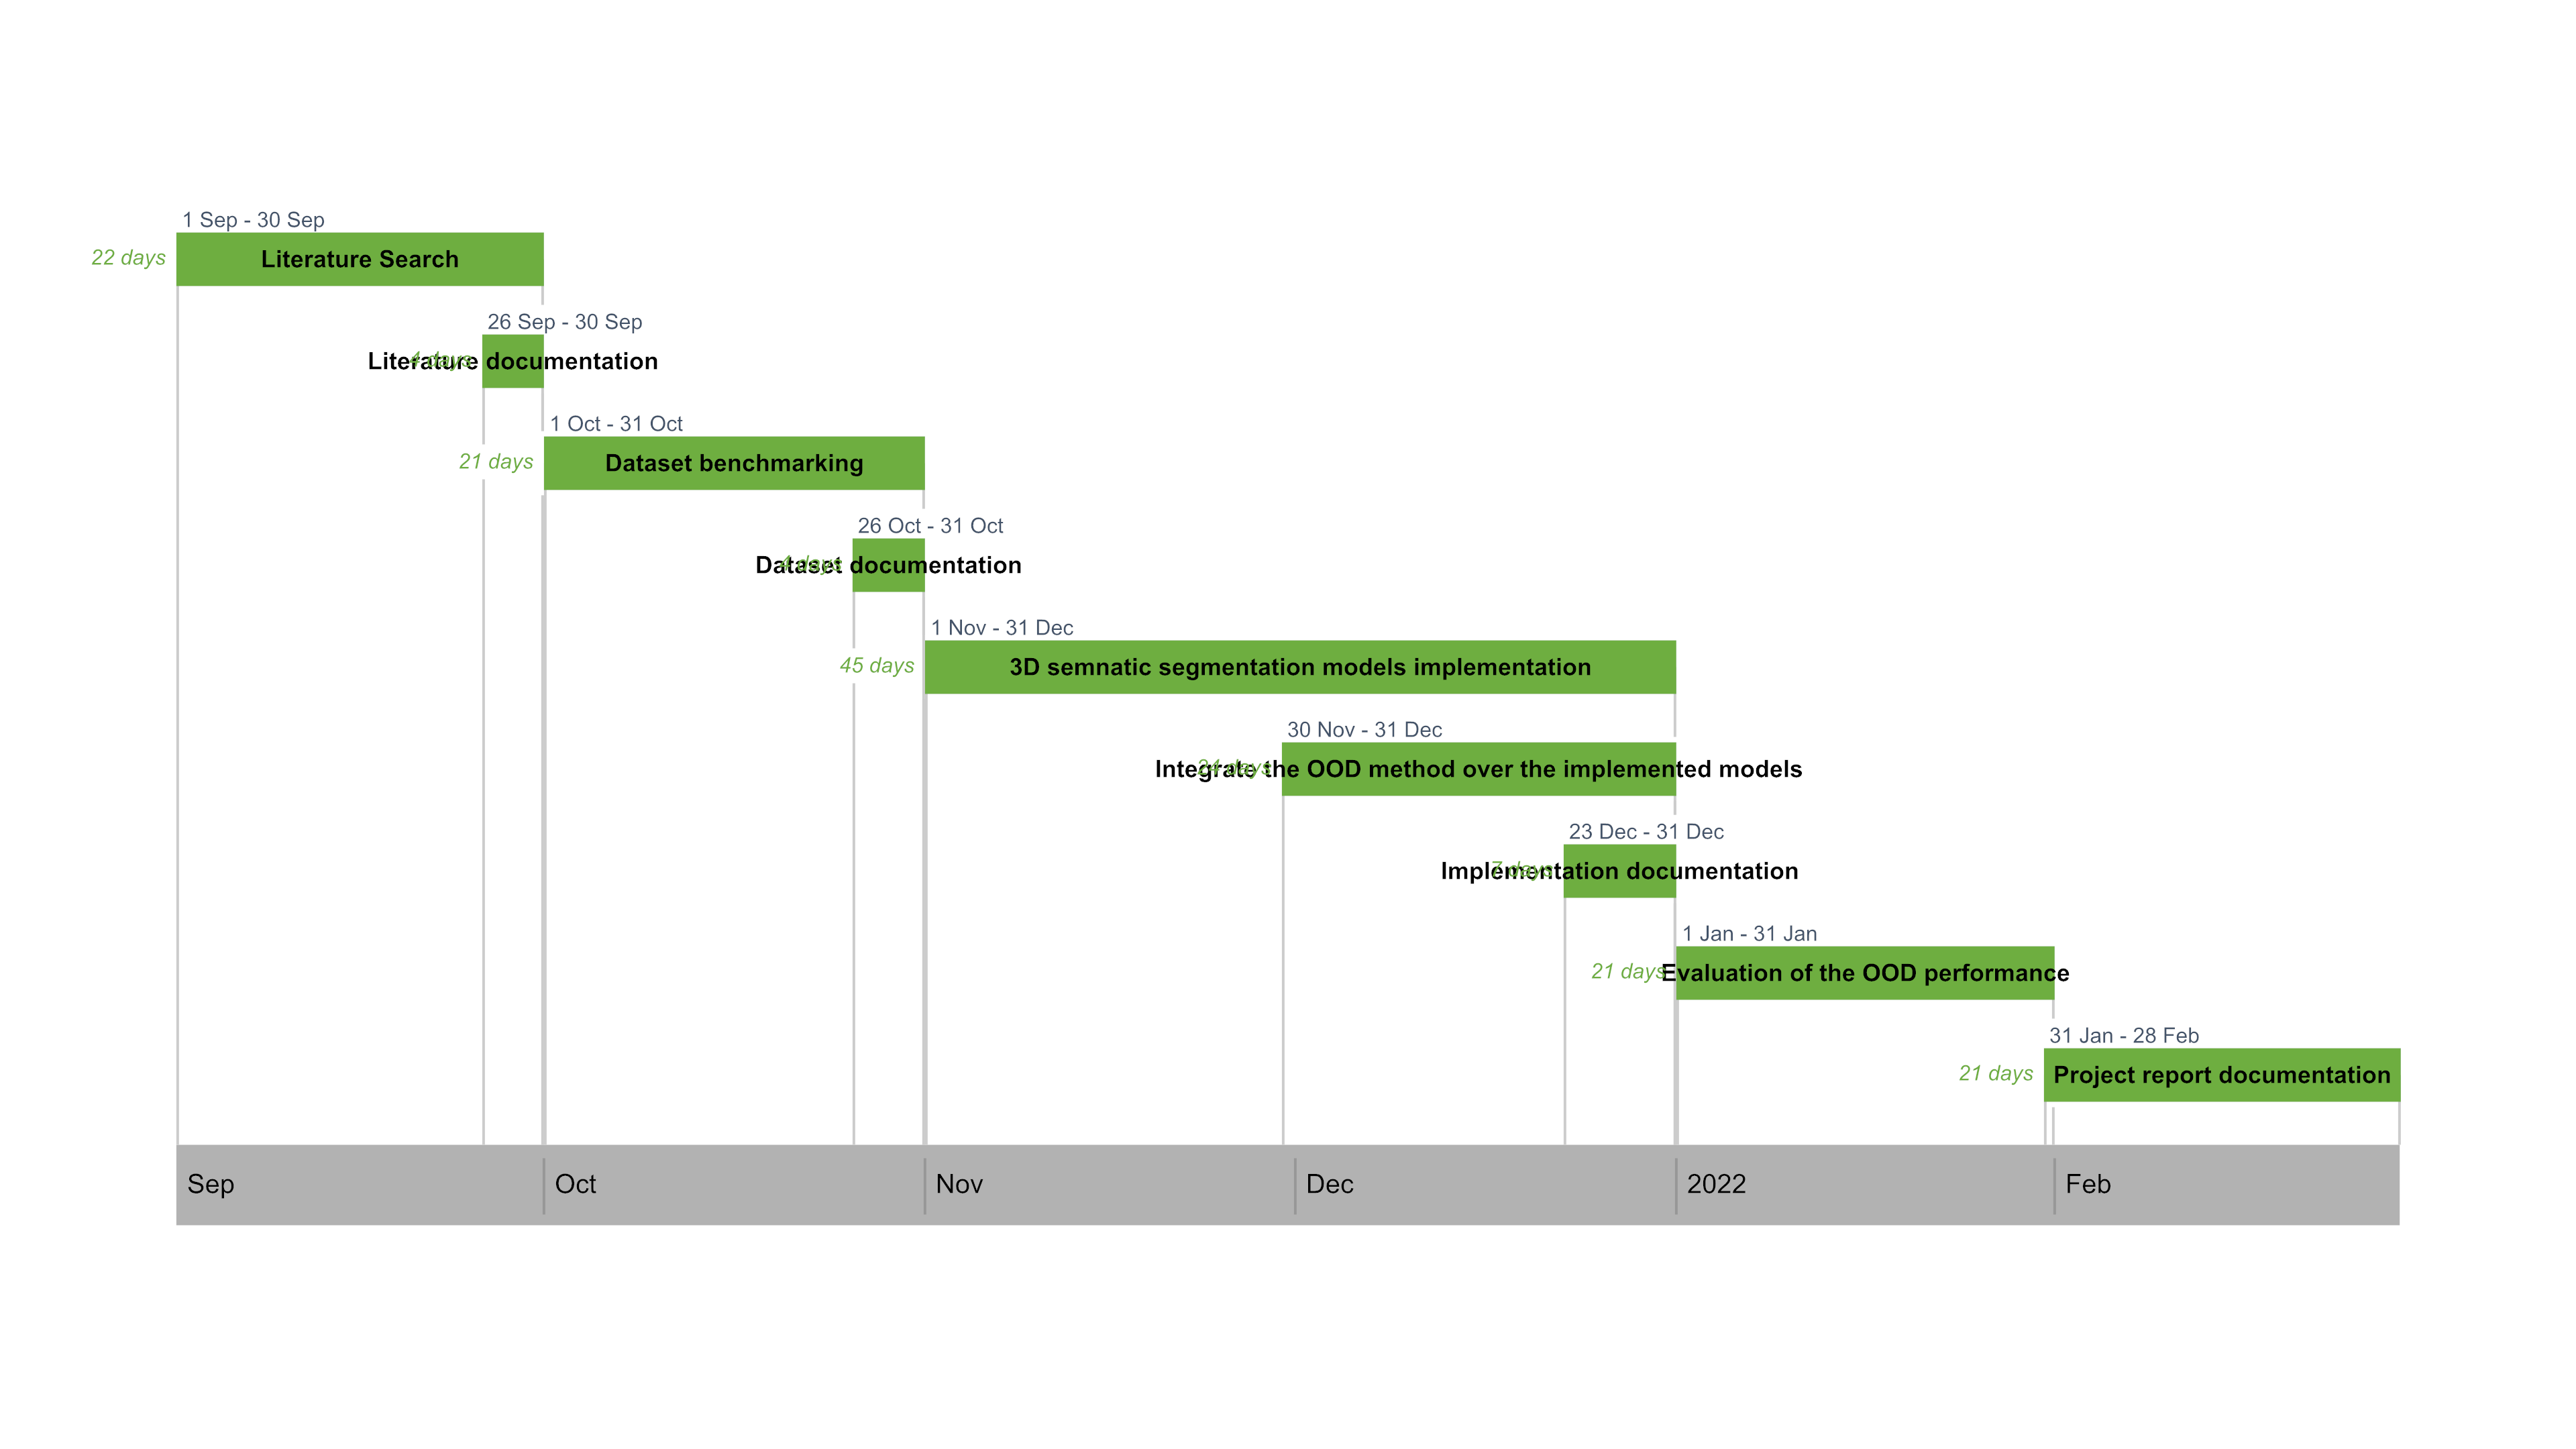
\includegraphics[scale=0.16]{images/rnd_deliverable_timeline}
    % 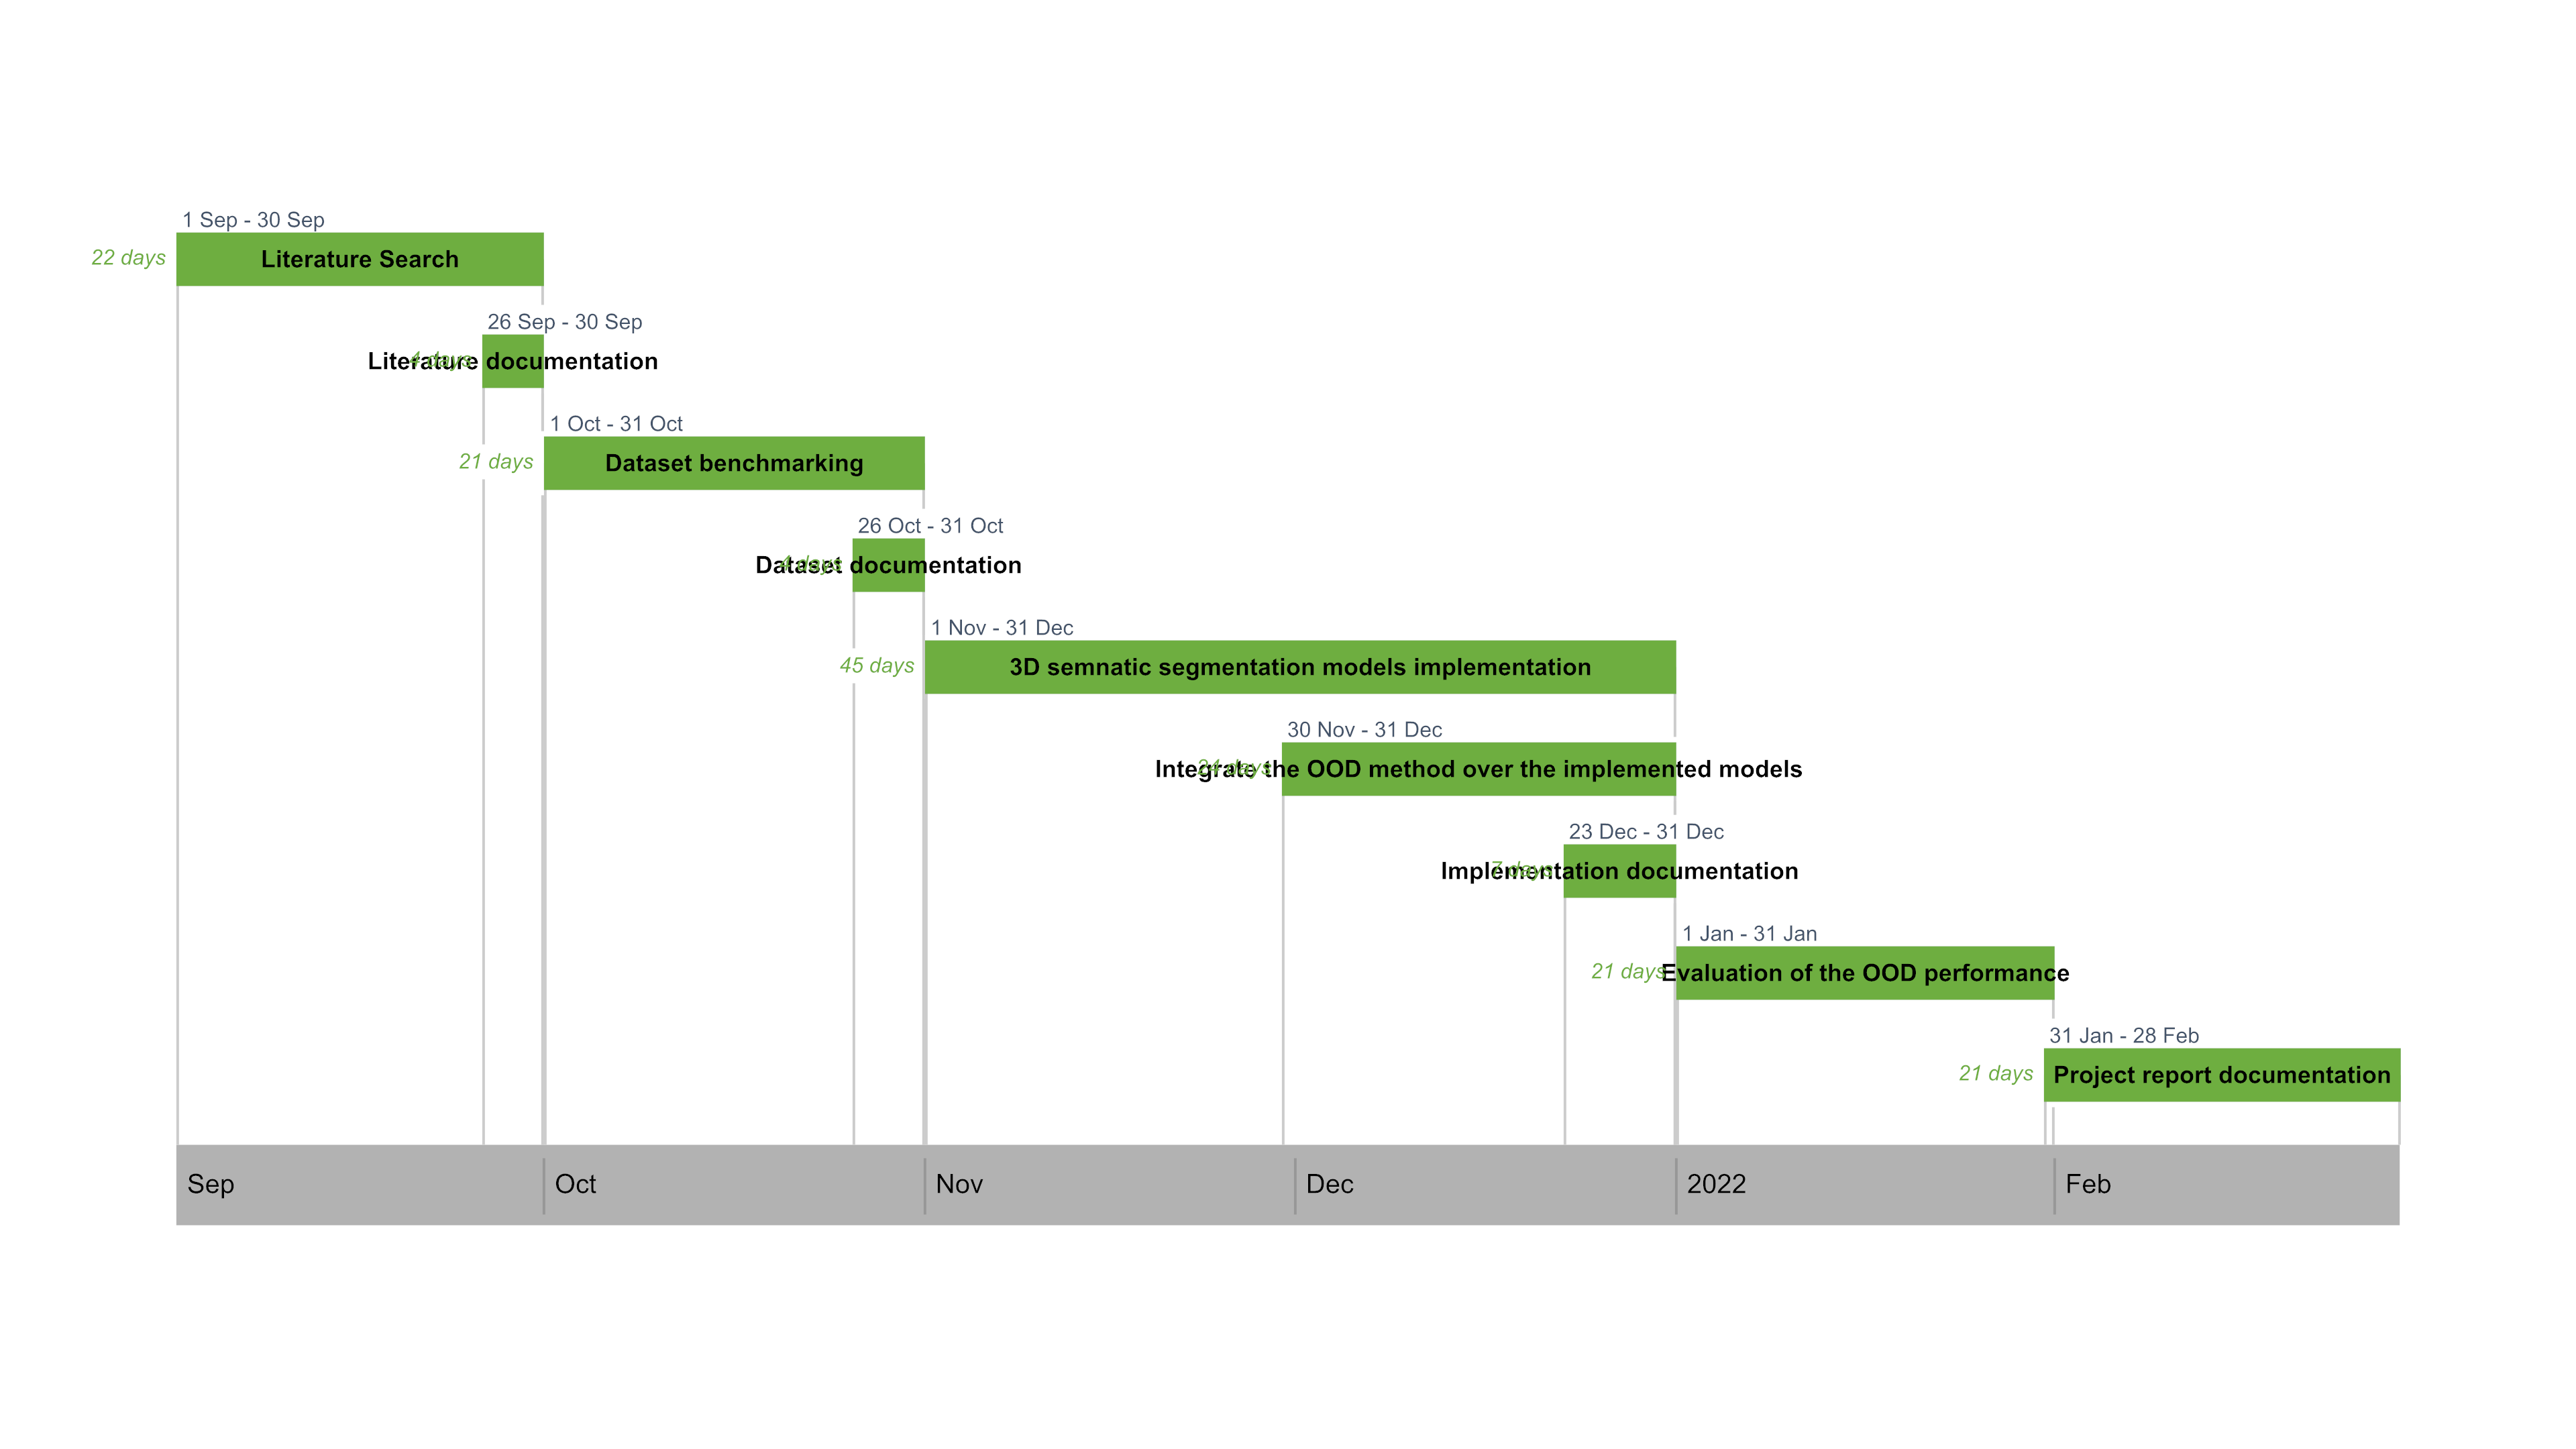
\includegraphics[width=\textwidth]{images/rnd_deliverable_timeline}
    \label{fig:schedl}
\end{figure}

\nocite{*}

% \bibliographystyle{plainnat} % Use the plainnat bibliography style
\bibliographystyle{abbrv}
\bibliography{bibliography.bib} % Use the bibliography.bib file as the source of references




\end{document}
